%!TEX root = main.tex
\section{Actionable VQS features for scientific insight (RQ3)} \label{VQS_features_discussion}
\tvcg{\subsection{Top-down v.s. Bottom-up analysis}}
To contextualize our study results with respect to prior work on how analysts make sense of data, we employ Pirolli and Card's~\cite{Pirolli} information foraging framework for domain-experts. Pirolli and Card's notional model distinguishes between information processing tasks that are \textit{top-down} \cut{(from theory to data)} and \textit{bottom-up} \cut{(from data to theory)}. \tvcg{Recent work in have also used the top-down v.s. bottom-up framework in understanding visualization construction\cite{Mendez2017}. In the context of visualization querying, top-down approaches are attribute-level specification to a query or an action, whereas bottom-up approaches originates from the data (or equivalently, the visualization).} 
\tvcg{\subsubsection{Querying Behavior}}
\par Our interactions with the scientists showed that different modalities for inputting a query can be useful for different problem contexts. \tvcg{To our surprise, despite the prevalence of sketch-to-query systems in literature, only two out of our nine users had a practical usage for query by sketching.} Overall, \tvcg{we found that} bottom-up querying via drag-and-drop was more intuitive and commonly used than top-down querying \tvcg{methods, such as} sketching or input equations. 
\par The main reasons why participants did not find sketching useful was that they often do not start off their analysis with a pattern in mind. Later, their intuition about what to query is derived from other visualizations that they see in the VQS, in which case it made more sense to query using those visualizations as examples directly (via drag-and-drop). In addition, even if a user has a query pattern in mind, sketch queries can be ambiguous \cite{correll2016semantics} or impossible to draw by sketching (e.g. A2 looked for a highly-varying signal enveloped by a sinusoidal pattern indicating planetary rotation). 
\tvcg{\par The latter case is also evident from the unexpected use cases where sketching was simply used as a mechanism to modify the drag-and-dropped queries. As shown in Figure \ref{query_modification} top, M2 first sketched a pattern to find solvent classes with anticorrelated properties. However, the sketched query did not return the visualization he was interested in. So, he instead dragged and dropped one of the peripheral visualizations that was close enough to his desired visualization to the sketchpad and then smoothed out the noise due to outliers datapoints by tracing a sketch over the visualization. M2 repeated this workflow twice in separate occurrences during the study and was able to derive insights from the results. Likewise, A3 was interested in pulsating stars characterized by dramatic changes in amplitudes in the light curves. During the search, hotspots on stellar surfaces often show up as false positives as they also result in dramatic amplitude fluctuations, but happen at a regular interval. On the VQS, A3 looked for patterns that exhibits amplitude variations, but also some irregularities. As shown in Figure \ref{query_modification} bottom, she first picked out a regular pattern (suspected star spot), then modified it slightly so that the pattern looks more irregular. 
\begin{figure}[ht!]
    \centering
    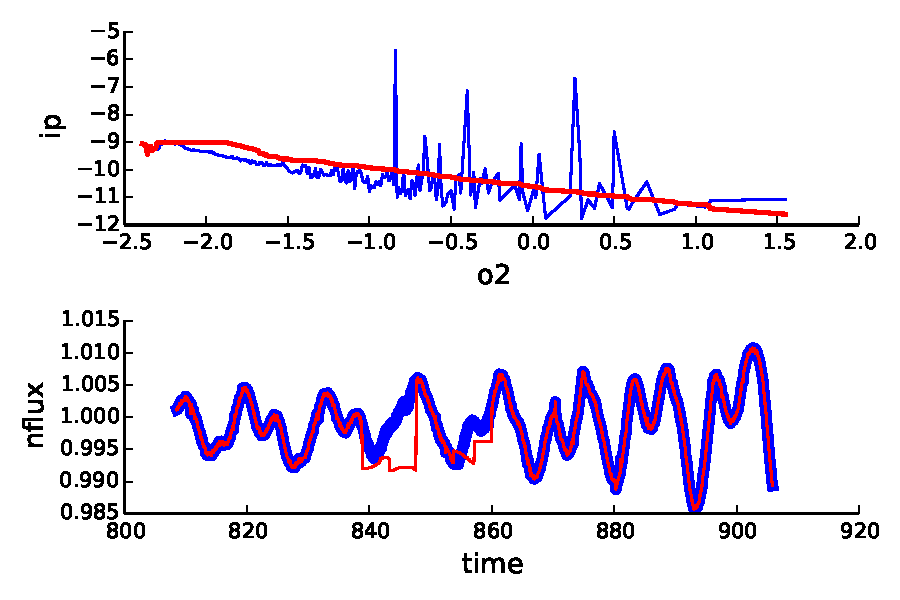
\includegraphics[width=\columnwidth]{figures/QueryModificationBySketch.pdf}
    \caption{\tvcg{Examples of query modification by M2 (top) and A3 (bottom) performed during the study The inital drag-and-dropped query is shown in blue and the sketch-modified queries is shown in red.}
    \label{query_modification}}
\end{figure}
\par Both of these use cases suggest that while sketching is an useful analogy for people to express their queries, the existing ad-hoc, sketch-only model for visualization querying is insufficient without data examples that can help analyst jumpstart their exploration. \emph{We suspect that this is why existing sketch-to-query systems are not commonly adopted in practice despite extensive research. This result, however, points to a potential need for high-level query modification interfaces that enable more precise visualization query specification in future VQSs.}} %This, however, points to an exciting direction for sketching interface in VQSs for developing advanced drawing and modification tools that enable more precise visualization query specification.}
\par Despite functional fitting being common in scientific data analysis, Figure \ref{feature_heatmap} shows that querying by equation is also unpopular for the same reason as a sketched query. In addition, the visualizations for both \astro and \bio exhibit complex processes that could not be written down \tvcg{as an equation} analytically. However, even when analytical relationships do exist (in the case of \matsci), it is challenging to formulate functional forms in an \tvcg{prescriptive,} ad-hoc manner. %For instance, \matsci discovered a known inverse relationship during exploration
%Which is really interesting. Which is something that we observed experimentally also. That is an interesting insight right htere. This seems to suggest that there is a fundamental issue in if you want to try to get better on this axis, and get as low as possible, you lose out on the other axis.
%once they see it they know it but they don't know beforehand
\par \tvcg{In contrast, when we looked at bottom-up querying approaches}, drag-and-drop was the querying mechanism used most frequently by the participants. Examples of practical uses of drag-and-drop includes inspecting the top-most similar visualizations that lie in a cluster and finding visualizations that are similar to an object of interest that exhibits the desired pattern. \tvcg{Likewise,} many participants envisioned use cases for pattern loading. \tvcg{The ability to load in data patterns as a query would enable users to compare} visualizations between different experiments, species, or surveys, querying with known patterns from an external reference catalog (e.g. important genes of interest, objects labeled as supernovae) \tvcg{or verify} the results of a simulation or downstream analysis by finding similar patterns in their existing dataset. \tvcg{In addition, users can also specify} a more precise query that captures \tvcg{the essential shape features of a desired pattern} (e.g. amplitude, width of peak), which can not be precisely drawn as a sketched pattern. \tvcg{For example, as shown in the top left diagram in Figure \ref{example}, the width of the light curve is characteristic to the type of supernovae that its associated with and is therefore helpful for distinguishing the queried pattern from noise.}
\par While the usage of each querying feature may vary from one participant to the next, generally,  drag-and-drop and pattern upload are considered bottom-up approaches that go from data to theory by enabling users to query via examples of known visualizations. For top-down approaches such as query by sketching and input equations, the user starts with \tvcg{an intuition about how their desired patterns should look like based on theory, then queries based on that}. Our results indicate that \emph{bottom-up querying approaches are preferred over top-down when the users have no desired patterns in mind}, which is commonly the case for exploratory data analysis.
% \paragraph{Both top-down and bottom-up faceted exploration enable users to derive insights through VQSs.} 
%\subsection{Top-down and bottom-up faceted exploration} 
\tvcg{\subsubsection{Faceted Exploration Behavior}}
\par All participants either envisioned a use case or utilized \tvcg{the data faceting functionalities offered in \zv (filtering,  dynamic class)} to explore and compare subsets of their data. 
\par A1 expressed that even though the filtering step could be easily done programmatically on the dataset and reloaded into \zv, the filter constraint was a powerful way to dynamically test their hypothesis. Interactive filtering lowers the barrier between the iterative hypothesis-then-compare cycle, thereby enabling participants to test conditions and tune values that they would not have otherwise modified as much.
% echoing our previous finding that segmented workflow prevents extensive exploration.
During the study, participants used filtering to address questions such as: ``Are there more genes similar to a known activator when we subselect only the differentially expressed genes (e.g. DIFFEXP=1)?'' (G2) or ``Can I find more supernovae candidates if I query only on objects that are bright and classified as a star (e.g. flux\textgreater
10 AND CLASS\_STAR=1)?'' (A1). Three participants had also used filtering as a way to pick out individual objects of interest to query with. For example, G2 set the filter as gene=`9687' and explained \tvcg{that because ``
this gene is regulated by the estrogen receptor, when we search for other genes that resembles this gene, we can find other genes that are potentially affected by the same factors.''}
As shown in Figures \ref{action_heatmap} and \ref{feature_heatmap}, participants with the top-most provoked data actions (A1, A3, G2) made heavy use of filtering to explore different subsets of the data. 
\par While filtering enabled users to narrow down to a selected data subset, dynamic class creation enabled users to compare the relationships between multiple physical attributes and between subgroups of data. For example, M2 divided the solvents in the database to eight different classes based on the voltage properties, state of matter at room temperature, and viscosity levels, by dynamically setting the cutoff values to create these classes. By exploring the created custom classes, M2 learned that the relationship between viscosity and lithium solvation energy is independent of whether a solvent belongs to the class of high voltage or low voltage solvents. M2 cited that dynamic class creation was central to learning about this previously-unknown property of these two attributes: 
\begin{quote}
All this is really possible because of dynamic class creation, so this allows you to bucket your intuition and put that together. [...] I can now bucket things as high voltage stable, liquid stable, viscous, or not viscous and start doing this classification quickly and start to explore trends. [...] And look how quickly we can do it! Quite good!
\end{quote}
\par Participants employed \emph{a mix of bottom-up and top-down approaches when faceting through data in VQS}, including narrowing the search space based on some intuition about a phenomena, selecting individual visualizations, or specifying high-level groupings to compare and query with.
%selectively finding high-level grouping to compare and query with
% This was a finding that M2 have not previously One participant discovered that certain physical properties were decoupled from the high voltage properties of solvents. ``These properties are decoupled from the high voltage properties which is something that makes a whole lot of sense.'' When asked if he knew of this fact, he replied  ``Probably not. I mean I could have guessed. But [...] I would not have conclusively said that this is obvious.'' The same participant voluntarily described this feature in his own word:
% Simmilarly, on two different ----- radius of ---, be
% bright objects and -----. 
% Dynamic classes enabled 
% \par For a similar reason, cold-start problem is difficult for top-down approaches. input equations as query was an unpopular choice since both astronomy and biology had complex processes that could not be written down analytically. Only one of our participant used it ---, fammilar with functional fitting 
% this was surprising as functional fitting is a common procedure conducted in scientific analysis, but it is not suited for querying a visualization. 
% \par  \textbf{Cold-start problem:}
% One of the ---- coming up with what to query 
% In the control panels, --- however, Novices often don't have an idea of what to try 
% Interaction wise some participants wanted ----, 
% instruction manual showcasing examples of when and how each data ---- should be used. 

% peripheral viewing of visualization ----
% Another ----- , cold-start problem --- multiples of visualizations provided a way for ----- cold start problem. a lot of learning happening if this is a new dataset. All of except one our users have found outliers 
% (the last user used the results pane to scroll through and browse data with the default query)
% 2 out of the 5 datasets that participants used in the user study were preliminary dataset that had minimal data cleaning and transformations. 

% \par \textbf{Information Foraging in VQS:}

\subsubsection{Novel workflows focusing on one central foraging act.}\label{novel_workflow_foraging}
\par Pirolli and Card's notional model further characterize the trade-offs between three central activities in the information foraging process: exploring, enriching, and exploitingd~\cite{Pirolli}. \textit{Exploring} involves gathering more information during the analysis. \tvcg{In the context of VQSs}, exploring includes viewing representatives and outliers, incidental viewing of other visualizations \tvcg{in the ranked search results}, and querying via drag-and-drop and pattern-loading. \textit{Enriching} involves tasks that narrow down the space of analysis, such as filtering, dynamic class creation, query specification, and querying via input equations and sketching. \textit{Exploiting} involves spending time inspecting the results in more detail, including interpreting each visualization in greater detail or making plotting changes that offer another perspective (smoothing, display, and interpretability settings). %\dor{This paragraph was moved from beginning of Sec 6 to here, the notion of bottom up and top down is removed in this discussion to avoid confusion.}
% Given these observations on how users make use features, we discuss some of the unexpected workflows that the users have constructed to fit their use cases that made use of many features in VQS. Workflow that the participants contructed within \zv consist of ---- multiple interactions, settings ,queries , .etc that work together to a larger high-level goal. 
\par In addition to \tvcg{observing} how participants use features within \tvcg{the VQS}, we also find that participants often create unexpected workflows that chain together multiple \tvcg{analysis steps, including} interactions, controls, and queries in order to address a higher-level research question. These behaviors can be explained in terms of the foraging acts \tvcg{proposed by Piroli and Card.} We find that participants often construct a central workflow, \tvcg{which they then iterate on while adding additional variations.} \ccut{then they continue to perform the same workflow over and over with additional variations.} Their \emph{central workflow often resembles one of the three foraging acts} that aligns with the type of research question and dataset they are interested in. The variations are based on intermixing their central workflow with the other two foraging \tvcg{acts}.
% We find that participants often have a strong inclination to perform tasks that resembles one of the three foraging act and sparsely intermixed with other activities to support their analysis, depending on the type of research question and dataset they are interested in.
\par  For example, the geneticists were mostly interested in \textit{exploring} clusters to gain an overall sense what profiles exist in the dataset \tvcg{through representative trends} and therefore queried mainly through drag-and-drop. The variations to their main workflow include changing cluster sizes and display settings to offer them different perspectives on the dataset (\textit{exploit}) and filtering on data attributes (\textit{enriching}). 
%For example, G2 knew that there was three repeated measurements that was taken for every timestep, in one of the profiles there was a sharp jump whereas other datapoints are relatively flat, he then concludes by inspecting in the scatterplot view that the rise in gene expression is probably due to an experimental error rather than the activation of a gene, because the other two repeated measurements were similar in magnitude. In other words, the scatterplot view offered him density of points as another proxy to consider that was not offered in the line chart perspective.
The main workflow for the astronomers in our user study involves \textit{enriching}, either through the creation of groups or via filtering data subsets. The main workflow for \matsci involves \textit{exploiting}, since they spend the majority of their efforts performing ``close-reading'' of individual visualizations to understand the relationships between  physical variables. %This is true for both participants with and without a desired pattern in mind. For the participant without a desired pattern (G2), he created groups based on quartile statistics of additional data attributes and recorded the most significant representative pattern. 
% [---] out of 9 of our participants had more than one main workflow.
\ccut{\par Designing VQS features that diversifies potential variations and helps the creation of multiple analysis workflows that could expand the space of actions that could be performed during the analysis. Furthermore, the ability to construct these workflows within VQS relies that the users have a clear mental model for how the multiple coordinated views in the VQS interacts, as described by A2:
\begin{quote}
I like that [the VQS interface is] very clean, once you do it once or twice, you remember how this thing works. I used to know colleagues that use some software for light curve treatment and it's so full of options and suboptions that it is painful to use. In the end the software will not give you all the answers, but the analysis you made on your own.
\end{quote}
Proper explanation and documentation of the system's functionalities with examples is also crucial to help construct this mental model for how the VQS works, as G1 puts it as:
\begin{quote}
[The] features itself are good, but there should be a manual that gives examples and descriptions of each of the options and functionalities that could be done. If a person is unfamiliar with their dataset, they might not have think of which sets of operations to select, having these simple scenarios can sometimes ring a bell for them on what operations they could do. For example, when would have I do use a different similarity metric than Euclidean? When would it be good for me to view the data as a scatterplot rather than a line chart?
\end{quote}}

\tvcg{\subsection{The need for comparisons across multiple collections of visualizations on different data attributes.}}
\par All participants wanted the ability to perform comparisons across multiple collections of visualizations on different data attributes, including comparison tasks such as:
comparing between genes that belong to different functional groups (G1,G3); 
comparing between stars that harbor planets (which exhibits a transit pattern) and stars that don't (A2);
comparing similarity and dissimilarity between two different sets of y measurements, such as time series of gene expression v.s. hypersensitivity (G2), stellar fluxes across different bands (A1); and comparing the correlation between different chemical properties for different solvent groups (M2).
\par These complex tasks are akin to the queries in the Zenvisage Query Language (ZQL)~\cite{Siddiqui2017}, which we did not demonstrate to our participants during the study to avoid confusion. \tvcg{Currently, to complete these tasks using \zv},  participants would have had to use the querying interface multiple times while also remembering past results, which can be error-prone. Developing sensible interactions to map user intentions to sophisticated query languages like ZQL is an important direction for future work. 
% % Multi-group comparison could be covered by ZQL too.
% % This finding also points to the need for supporting multidimensional attribute views in VQS, 

\subsection{Integrated workflow results in more experimentation.}
\par Our participants' original workflow often requires them to compare between many visualizations manually through separate analysis and visualization steps. \ccut{The segmented analyze-then-visualize workflow is a common practice adopted by scientists who are used to thinking about visualizations as the final product of an analysis, rather than something used throughout the process to obtain insights. \cut{Since some statistical analysis can take a long time to compute, analysts often store their results separately and then visualize them with a separate module, so that ``cosmetic'' plotting changes could be applied more easily without recomputing.}} Three of the participants cited that this artificial segmentation was one of their chief bottlenecks. The cognitive overhead from the segmented workflow made them more hesitant to visualize the results of different parameters and data operations, as A2 noted:
\begin{quote}
The quick visualization is something that I could not do on my current framework. I could not query as fast as you do; I need to wait for it, plot, and then compare. Every time I plot, I need to define subplots for 12 visualizations, then its slower. That's the reason why I sometimes plot less, and I rely more on the statistics from the likelihood tests. Sometimes I plot less than I really should be doing.
\end{quote}
In Figure \ref{action_heatmap}, we also see that \zv provoked users to generate many data operations (PD) and hypotheses (PS).
\subsection{Rapid insights via VQSs catalyze new questions, hypotheses, and actions.}
\par \tvcg{The ability to rapidly experiment with large numbers of hypotheses in real time is a crucial step in the agile creative process in helping analysts discover actionable insights~\cite{Shneiderman2007a}. Five out of nine participants discussed how the dynamic, interactive update of the visualization in \zv was the main advantage for using VQSs over their original workflow.}
\par A common theme that we found across the \bio participants is that they often gain their intuition about the data from the representative trends. One example of rapid insight discovery comes from G1, G2, and G3, who first identified that the three representative patterns shown in \zv---induced genes (profiles with expression levels staying up), repressed genes (started high but went down), and transients (go up and then come down at different time points)---corresponded to the same three groups of genes discussed in a recent publication\cite{Gloss2017}. 
\par The clusters provoked G2 to generate a hypothesis regarding the properties of transients: \textit{``Is that because all the transient groups get clustered together, can I get sharp patterns that rise and ebb at different time points?''} To verify this hypothesis, G2 increased the parameter controlling the number of clusters and noticed that the cluster no longer exhibited the clean intuitive patterns he had seen earlier. G3 expressed a similar sentiment and attempted to identify different clusters. He proceeded by inspecting the visualizations in the cluster via drag-and-drop and found a group of genes that all transitioned at the same timestep, while others transitioned at different timesteps. G3 described the process of using VQSs as doing ``detective work'' that provoked him to generate further scientific hypotheses as well as data actions.